% Standalone figure for the Statistical Mechanics notes.
% Build: pdflatex quadruple.tex  (or run build.sh in this folder)
\documentclass[11pt,tikz,border=2pt]{standalone}
\usepackage{amsmath,amssymb}
\usetikzlibrary{arrows.meta, positioning}
\begin{document}
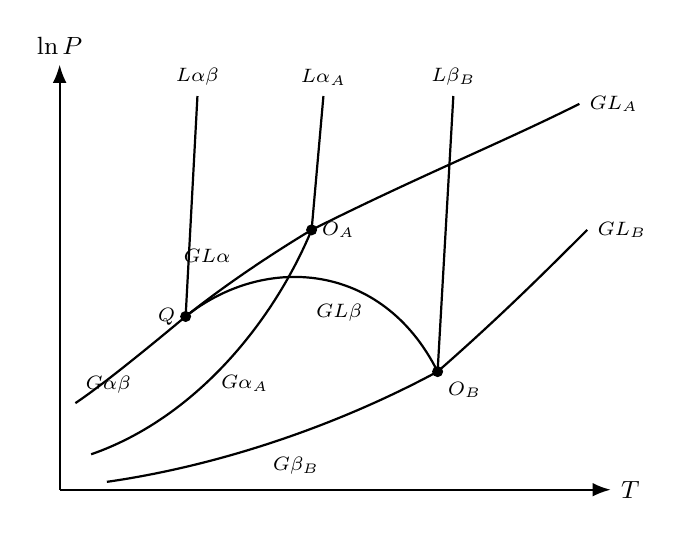
\begin{tikzpicture}[font=\small, >=Latex, line width=0.8pt]
    % axes
    \draw[->] (0,0) -- (7,0) node[right] {$T$};
    \draw[->] (0,0) -- (0,5.4) node[above] {$\ln P$};
    % quadruple point and triple points (schematic)
    \coordinate (Q) at (1.6,2.2);
    \coordinate (OA) at (3.2,3.3);
    \coordinate (OB) at (4.8,1.5);
    % quadruple curves
    \draw (Q) -- (1.75,5.0) node[above, font=\scriptsize] {$L\alpha\beta$};
    \draw (Q) .. controls (1.0,1.7) and (0.5,1.3) .. (0.2,1.1)
        node[above right, font=\scriptsize] {$G\alpha\beta$};
    \draw (Q) .. controls (2.1,2.6) and (2.7,3.0) .. (OA);
    \draw (Q) .. controls (2.6,3.0) and (4.1,2.9) .. (OB);
    \node[font=\scriptsize, above left] at (2.3,2.75) {$GL\alpha$};
    \node[font=\scriptsize] at (3.55,2.25) {$GL\beta$};
    % triple curves of A
    \draw (OA) -- (3.35,5.0) node[above, font=\scriptsize] {$L\alpha_A$};
    \draw (OA) .. controls (4.6,4.0) and (5.6,4.4) .. (6.6,4.9)
        node[right, font=\scriptsize] {$GL_A$};
    \draw (OA) .. controls (2.7,2.1) and (1.7,0.9) .. (0.4,0.45);
    \node[font=\scriptsize] at (2.35,1.35) {$G\alpha_A$};
    % triple curves of B
    \draw (OB) -- (5.0,5.0) node[above, font=\scriptsize] {$L\beta_B$};
    \draw (OB) .. controls (5.6,2.2) and (6.2,2.8) .. (6.7,3.3)
        node[right, font=\scriptsize] {$GL_B$};
    \draw (OB) .. controls (3.5,0.8) and (2.0,0.3) .. (0.6,0.1);
    \node[font=\scriptsize] at (3.0,0.3) {$G\beta_B$};
    % points
    \fill (Q) circle (2pt) node[left, font=\scriptsize] {$Q$};
    \fill (OA) circle (2pt) node[right, font=\scriptsize] {$O_A$};
    \fill (OB) circle (2pt) node[below right, font=\scriptsize] {$O_B$};
\end{tikzpicture}
\end{document}
